%%%%%%%%%%%%%%%%%%%%%%%%%%%%%%%%%%%%%%%%%%%%%%%%%%%%%%%%%%%
\begin{frame}\frametitle{Test}
As you have come so far, lets see if you can solve the following:

\begin{itemize}
% \item How would you find a minimum of $y=e^(2 - x) + x^2 - x/2$?
% \item Transformers: can you have 5 attention heads with a sequence length equal to 100 and embedding dimension to 512, and why?
\item Please explain why the Bellman Equation is important and explain how you have used it in your work.
\item DQN RL: how can you use DQN on an environment with 100 unique states, and actions taking values on the interval $[-0.5, 0.5]$?
\end{itemize}

{\tiny (Ref: ``Reinforcement Learning Expert'' - MSBAI)}

If, there is a long way to go \ldots  Next are some of the learning resources \ldots
\end{frame}


%%%%%%%%%%%%%%%%%%%%%%%%%%%%%%%%%%%%%%%%%%%%%%%%%%%%%%%%%%%%%%%%%%%%%%%%%%%%%%%%%%
\begin{frame}[fragile]\frametitle{}
\begin{center}
{\Large References}
\end{center}
\end{frame}

%%%%%%%%%%%%%%%%%%%%%%%%%%%%%%%%%%%%%%%%%%%%%%%%%%%%%%%%%%%
\begin{frame}[fragile]\frametitle{Learning Resources}
\begin{center}
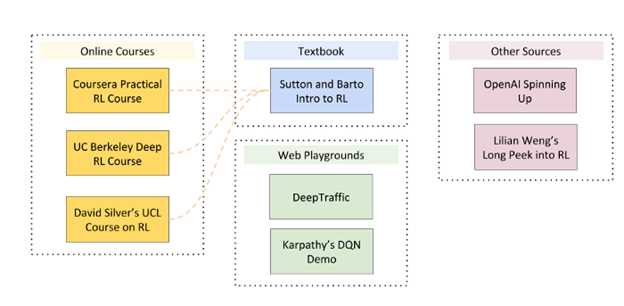
\includegraphics[width=\linewidth,keepaspectratio]{rl24}
\end{center}
{\tiny (Ref: Newbie’s Guide to Study Reinforcement Learning - Towards Data Science)}
\end{frame}

%%%%%%%%%%%%%%%%%%%%%%%%%%%%%%%%%%%%%%%%%%%%%%%%%%%%%%%%%%%
\begin{frame}\frametitle{References}
Many publicly available resources have been refereed for making this presentation. Some of the notable ones are:
\footnotesize
\begin{itemize}
\item Open AI Spinning Up - https://spinningup.openai.com/en/latest/index.html
\item Learning in Random Environments - Ekaba Bisong
\item Reinforcement Learning : Playing to Win - Shweta Bhatt
\item Deep Q Network, a deep reinforcement learning approach - Nitin Mukesh
\item Hugging Face Course https://github.com/huggingface/deep-rl-class
\item Deep Reinforcement Learning: CS 285 Fall 2020
\item RL Course by David Silver
\item Reinforcement Learning Specialization https://www.coursera.org/specializations/reinforcement-learning)
\item RLlib https://docs.ray.io/en/latest/rllib/index.html
\item IITM Reinforcement Learning http://www.cse.iitm.ac.in/~ravi/courses/Reinforcement%20Learning.html
\item Deep Reinforcement Learning Course, Fast Deep RL - Dibya Chakravorty
\end{itemize}
\end{frame}
